\newpage

\subsection{Configuration for code generation in Eclipse}
\genHeader

As there is already generated code (provided via a plugin in Eclipse) for the existing \textsf{GenModel} metamodel, we do \emph{not} want to export our
incomplete subset of \textsf{GenModel} in EA.

\begin{enumerate}
\item[$\blacktriangleright$] To prevent this, right-click the \textsf{GenModel} package in EA and select ``Properties/Moflon'' and change the tagged value
\texttt{Moflon::Export} to \texttt{false} (Fig.~\ref{fig_customNS}).
\end{enumerate}

Furthermore, we have to set the ``real'' name and URI of the project to be used in Eclipse so that references are exported properly. 
\begin{enumerate}
\item[$\blacktriangleright$] In the ``Properties/Moflon" dialogue for \textsf{GenModel}, create the new tagged values \texttt{Moflon::CustomNsPrefix} and
\texttt{Moflon::CustomNsUri} and set them according to Fig.~\ref{fig_customNS}.
These values can be determined by inspecting the corresponding values in the existing .ecore file (i.e.,~the existing metamodel).
\end{enumerate}

\begin{figure}[htbp]
\begin{center}  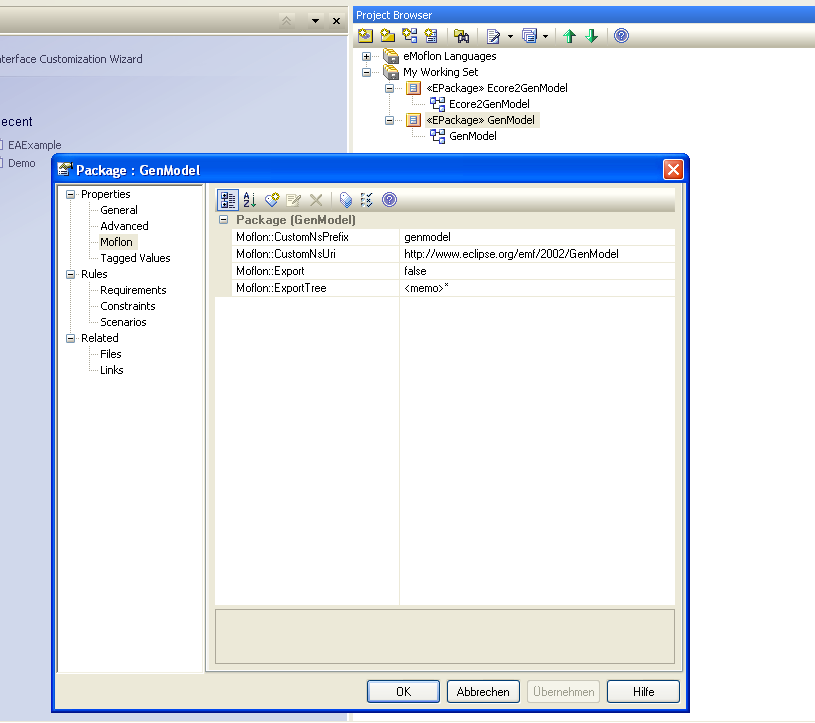
\includegraphics[width=0.87\textwidth]{8_nsUriPre}
  \caption{}  
  \label{fig_customNS}
\end{center}
\end{figure}

\begin{enumerate}
\item[$\blacktriangleright$] Export all projects as usual to your Eclipse workspace and update the metamodel project by pressing \textsf{F5}.

\item[$\blacktriangleright$] Convert the generated Eclipse project \texttt{Ecore2GenModel} to a \emph{plugin project} by right-clicking the project and
selecting ``Configure/Convert to Plug-in Projects...''. This makes it easier to set the required dependencies for code generation.

\item[$\blacktriangleright$] Now right-click \texttt{Ecore2GenModel} and choose ``Plug-in Tools/Open Manifest''.
In the window that opens up, choose the \texttt{Dependencies} tab, click \texttt{Add}, and type in \texttt{org.eclipse.emf.codegen.ecore} (which includes both
the \textsf{Ecore} and \textsf{GenModel} libraries as required).
\end{enumerate}

Although we have already specified the name and URI of the existing project (in our case \textsf{GenModel}) in EA, we now have to tell eMoflon where to find the
implementation (generated code) for the existing project.
\begin{enumerate}
\item[$\blacktriangleright$] Open the \texttt{moflon.properties} file located in your project folder and insert the following lines:\\
\texttt{{\tiny ADDITIONAL\_DEPENDENCIES=platform:/plugin/org.eclipse.emf.codegen.ecore/model/GenModel.ecore}}\\
\texttt{{\tiny ADDITIONAL\_USED\_GEN\_PACKAGES=platform:/plugin/org.eclipse.emf.codegen.ecore/model/GenModel.genmodel}}
\end{enumerate}

Finally, to compenstate for some cases where our naming conventions were violated, add the following mappings as corrections:

\begin{enumerate}
\item[$\blacktriangleright$] An \emph{import mapping} for correct generation of the required import:\\
\texttt{\tiny IMPORT\_MAPPINGS=genmodel-> org.eclipse.emf.codegen.ecore.genmodel}

\item [$\blacktriangleright$] A \emph{factory mapping} to ensure that \texttt{GenModelFactory} is used as the factory for creating elements in the
transformation instead of \texttt{Genmodel\-Factory}, which would be the default convention:\\
\texttt{\tiny FACTORY\_MAPPING=genmodel-> GenModelFactory}
\end{enumerate}

Your \textsf{moflon.properties} file should now closely resemble Fig.~\ref{fig_mofProp}. Now generate code once more for the project and ensure with a JUnit
test that the transformation behaves as expected.

\vspace{0.5cm}

\begin{figure}[htbp]
\begin{center}  %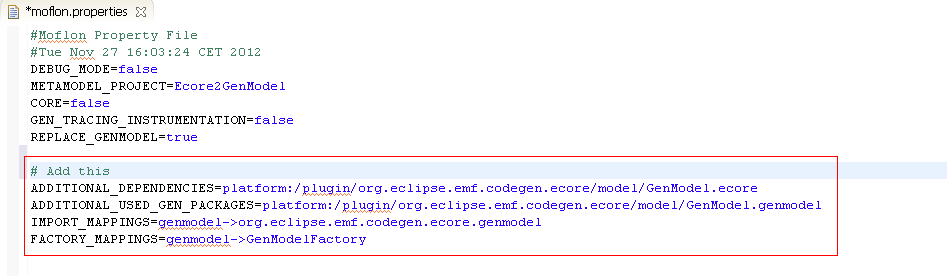
\includegraphics[angle=90,height=0.7\textheight]{9_mofProperties}
\hspace*{-2cm}
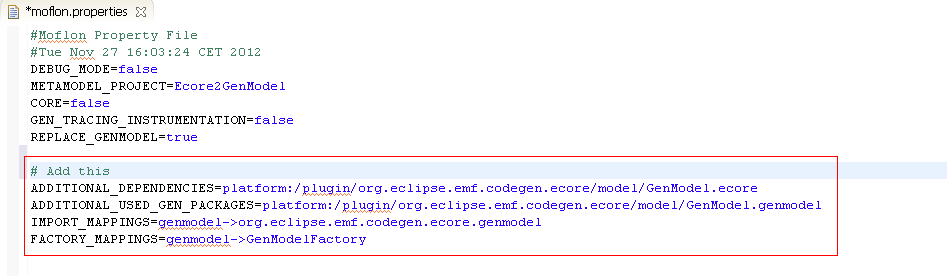
\includegraphics[width=1.5\textwidth]{9_mofProperties}
  \caption{Additional properties for code generation}  
  \label{fig_mofProp}
\end{center}
\end{figure} 
